
\chapter{3D Heat Transfer Methodology}

3D heat transfer simulation is a crucial aspect when designing, retrofitting, or analyzing an architectural envelope.
Simulation approaches enable modelers to understand and predict thermal comfort, providing detailed description visualization of heat flow, insulation performance, and energy efficiency. 
Furthermore, 3D simulations are more accurate than the traditional methods highlighted in the previous chapter. 
This way, users can detect and address complex issues such as thermal bridges and intricate geometric designs. 
This approach reduces the time, resources, and cost of identifying potential problems in the design of a building. 
 
This chapter showcases the workflow to build a 3D heat transfer approach integrated into the architects' modeling software to precisely model and optimize building envelopes, leading to better-informed decisions about insulation, material choice, and energy efficiency. The flowchart in \ref{fig:flowchart} is an overview of the 3D simulation steps. The following sections present the validation case, methodology, pre-processing, simulation setup, solver explanation, automation, post-processing, results, and finally the discussion. 






   
\begin{figure}[h!]
     \centering
    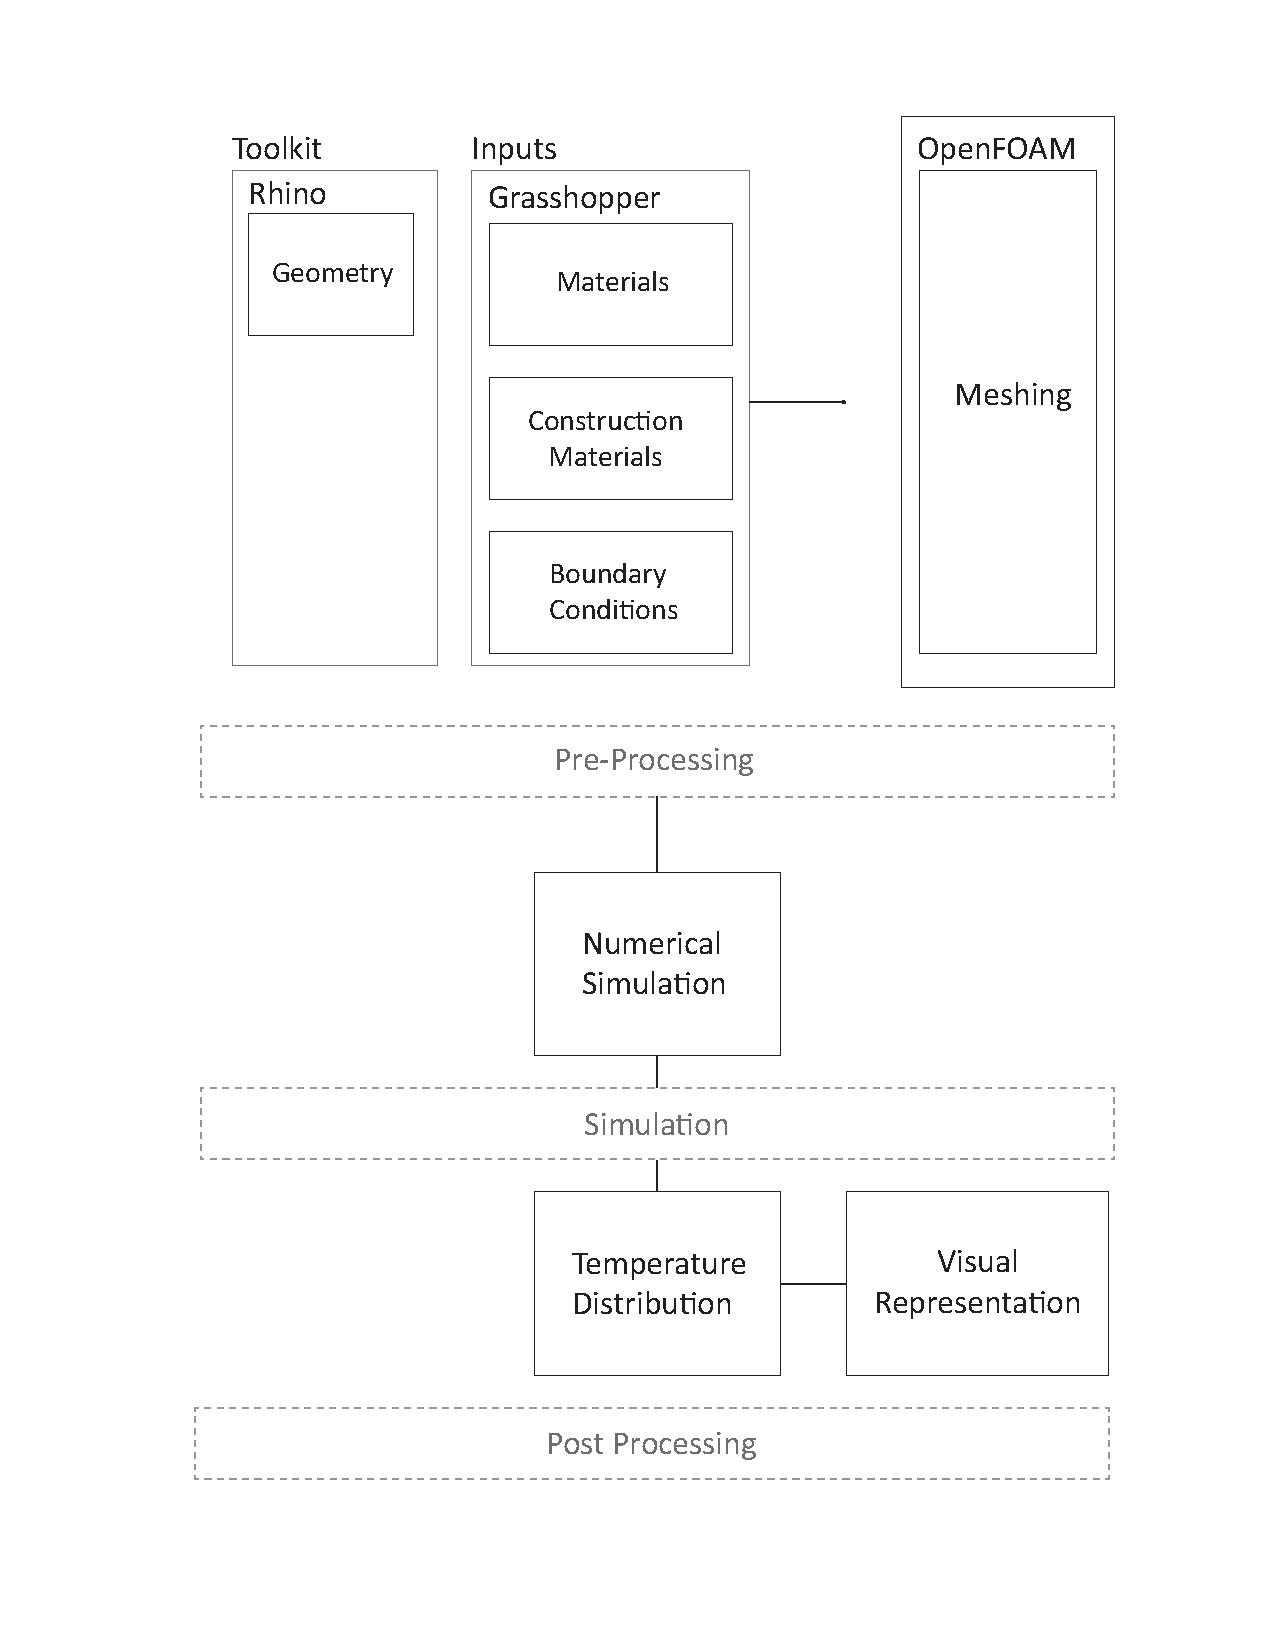
\includegraphics[trim=2.7cm 1.7cm 2.7cm 1.5cm, clip, width=0.7\linewidth]{Figures/flowchartv.pdf}
     \caption[Simulation Flowchart]{Flowchart of simulation steps starting from pre-processing to the post-processing of the simulation.}
   \label{fig:flowchart}
 \end{figure}



\subsubsection{Methodology Overview}
The first step in the methodology is to select a 3D validation case study to model in Rhino. 
Then, \gls{GH}  is used to create a script that bridges the gap between Rhino (the architectural modeling software) and  \gls{OF} (the CFD software package). A detailed description of the workflow, \gls{GH} automation, and the \gls{OF} solver are illustrated in the following sections.





\section{Validation Case Study}
The selected case is sourced from The International Organization for Standardization (ISO) \cite{ISO}. The case study is a validated 3D heat transfer case documented in \textit{ISO 10211:2007}\footnote{ISO 10211:2007---Thermal bridges in building construction. Validation of case A.3 \cite{ISO}.}. 
The geometry consists of two levels: a first floor and a second floor, separated by a floor slab and a plaster floor. The walls are composed of aerated concrete, insulation material, and brick.
A description of each material in the geometry can be found in \ref{fig:validation-case-materials} \textbf{(a)}.

%One of the challenges we faced was retrieving this case study due to the lack of availability of validated 3D and not 2D heat transfer cases that incorporate building materials. 
Beyond \textit{ISO 10211:2007}, it is also documented in the QuickField 6.6 (student version) software where the properties, layers, and boundary conditions of the materials are accessible, which we exported to compare it with our method. 

   


\begin{figure}[h!]
    \centering
    \begin{minipage}[t]{0.54\columnwidth}
        \centering
        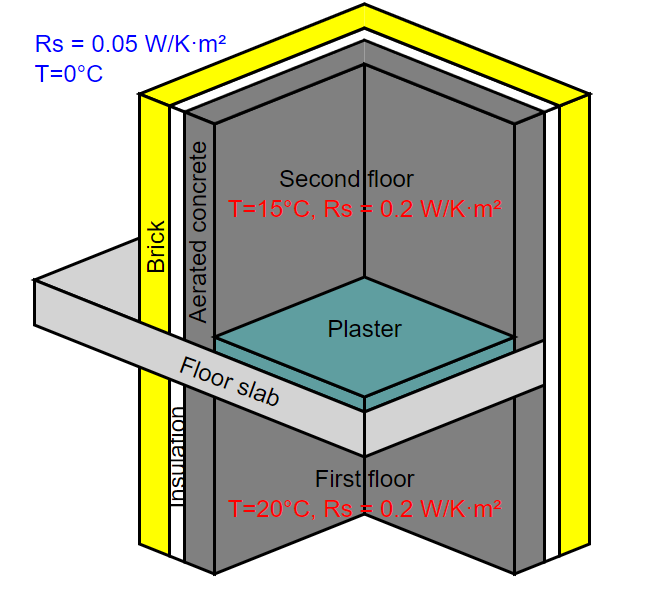
\includegraphics[width=\linewidth]{Figures/validationcase}
        \textbf{(a)}
    \end{minipage}
    \hfill
    \begin{minipage}[t]{0.8\linewidth}
        \centering
        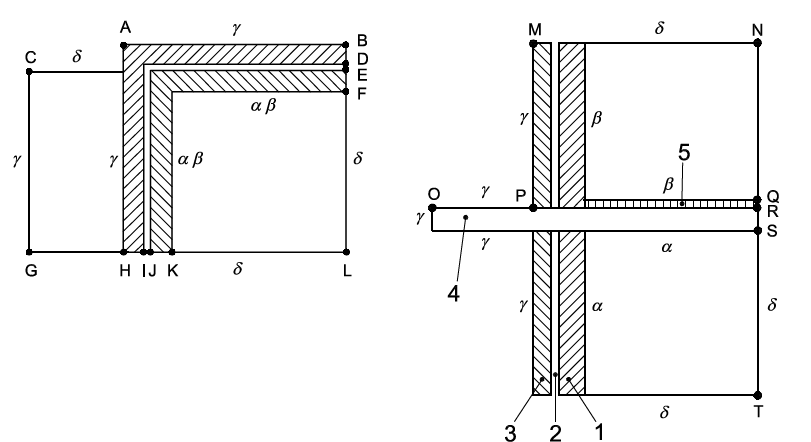
\includegraphics[width=\linewidth]{Figures/isodesc.png}
        \textbf{(b)}
    \end{minipage}
    
    \caption[3D Validation Materials]{\textbf{(a)} Validation case materials \cite{ISO}. \textbf{(b)}  Validation case sections retrieved from \gls{EN} ISO 10211:2007(E) \cite{ISO}.}
    \label{fig:validation-case-materials}
\end{figure}









QuickField's Heat Transfer module offers versatile features including steady-state and transient formulations with customizable initial field distributions and flexible time parameters, accommodating nonlinear specific heat and nonlinear or anisotropic properties. Although the results include diverse thermal field mappings such as temperature, heat flux, and thermal gradients, editing and customizing the post-process options and locations were limited.




\section{Rhino  Automation} %STOPPED HERE
After selecting the validation case, the geometry is modeled in Rhinoceros, where it will be used as a user interface to connect the model to \gls{GH}. \gls{GH} is a visual programming environment that we use to automate the \gls{OF} simulation. 
The \gls{GH} script enables the automation of the geometry pipeline, which, for example, enables us to find the coordinates of the points in the region, and to set the mesh, boundary conditions, and material properties. 
In addition, we use \gls{OF}, which is an open-source computational fluid dynamics (CFD) software package that is used to simulate fluid flow, heat transfer, and other capabilities. 


%\subsection{OF Text files Automation by  \gls{ \gls{GH}}}   
This subsection explains the Grasshopper script that automatically creates and exports STL files, defines material properties, finds the location of the points in the meshes, and writes all the text files needed to run the \gls{OF} case.

\subsubsection{Materials Properties Component}
The component shown in \ref{matgh} is a dictionary for the material connected to specific geometry. Each different zone in Rhino needs to be connected to the shown component by adding the corresponding specifications for the material such as name, type, temperature, specific heat capacity, thermal conductivity, and density. This component is considered the base and many other sections in the script depend on it, such as writing the other text files in 0 files where the boundary conditions are needed or writing the constant and system files. 


\begin{figure}[tbh]
\centering
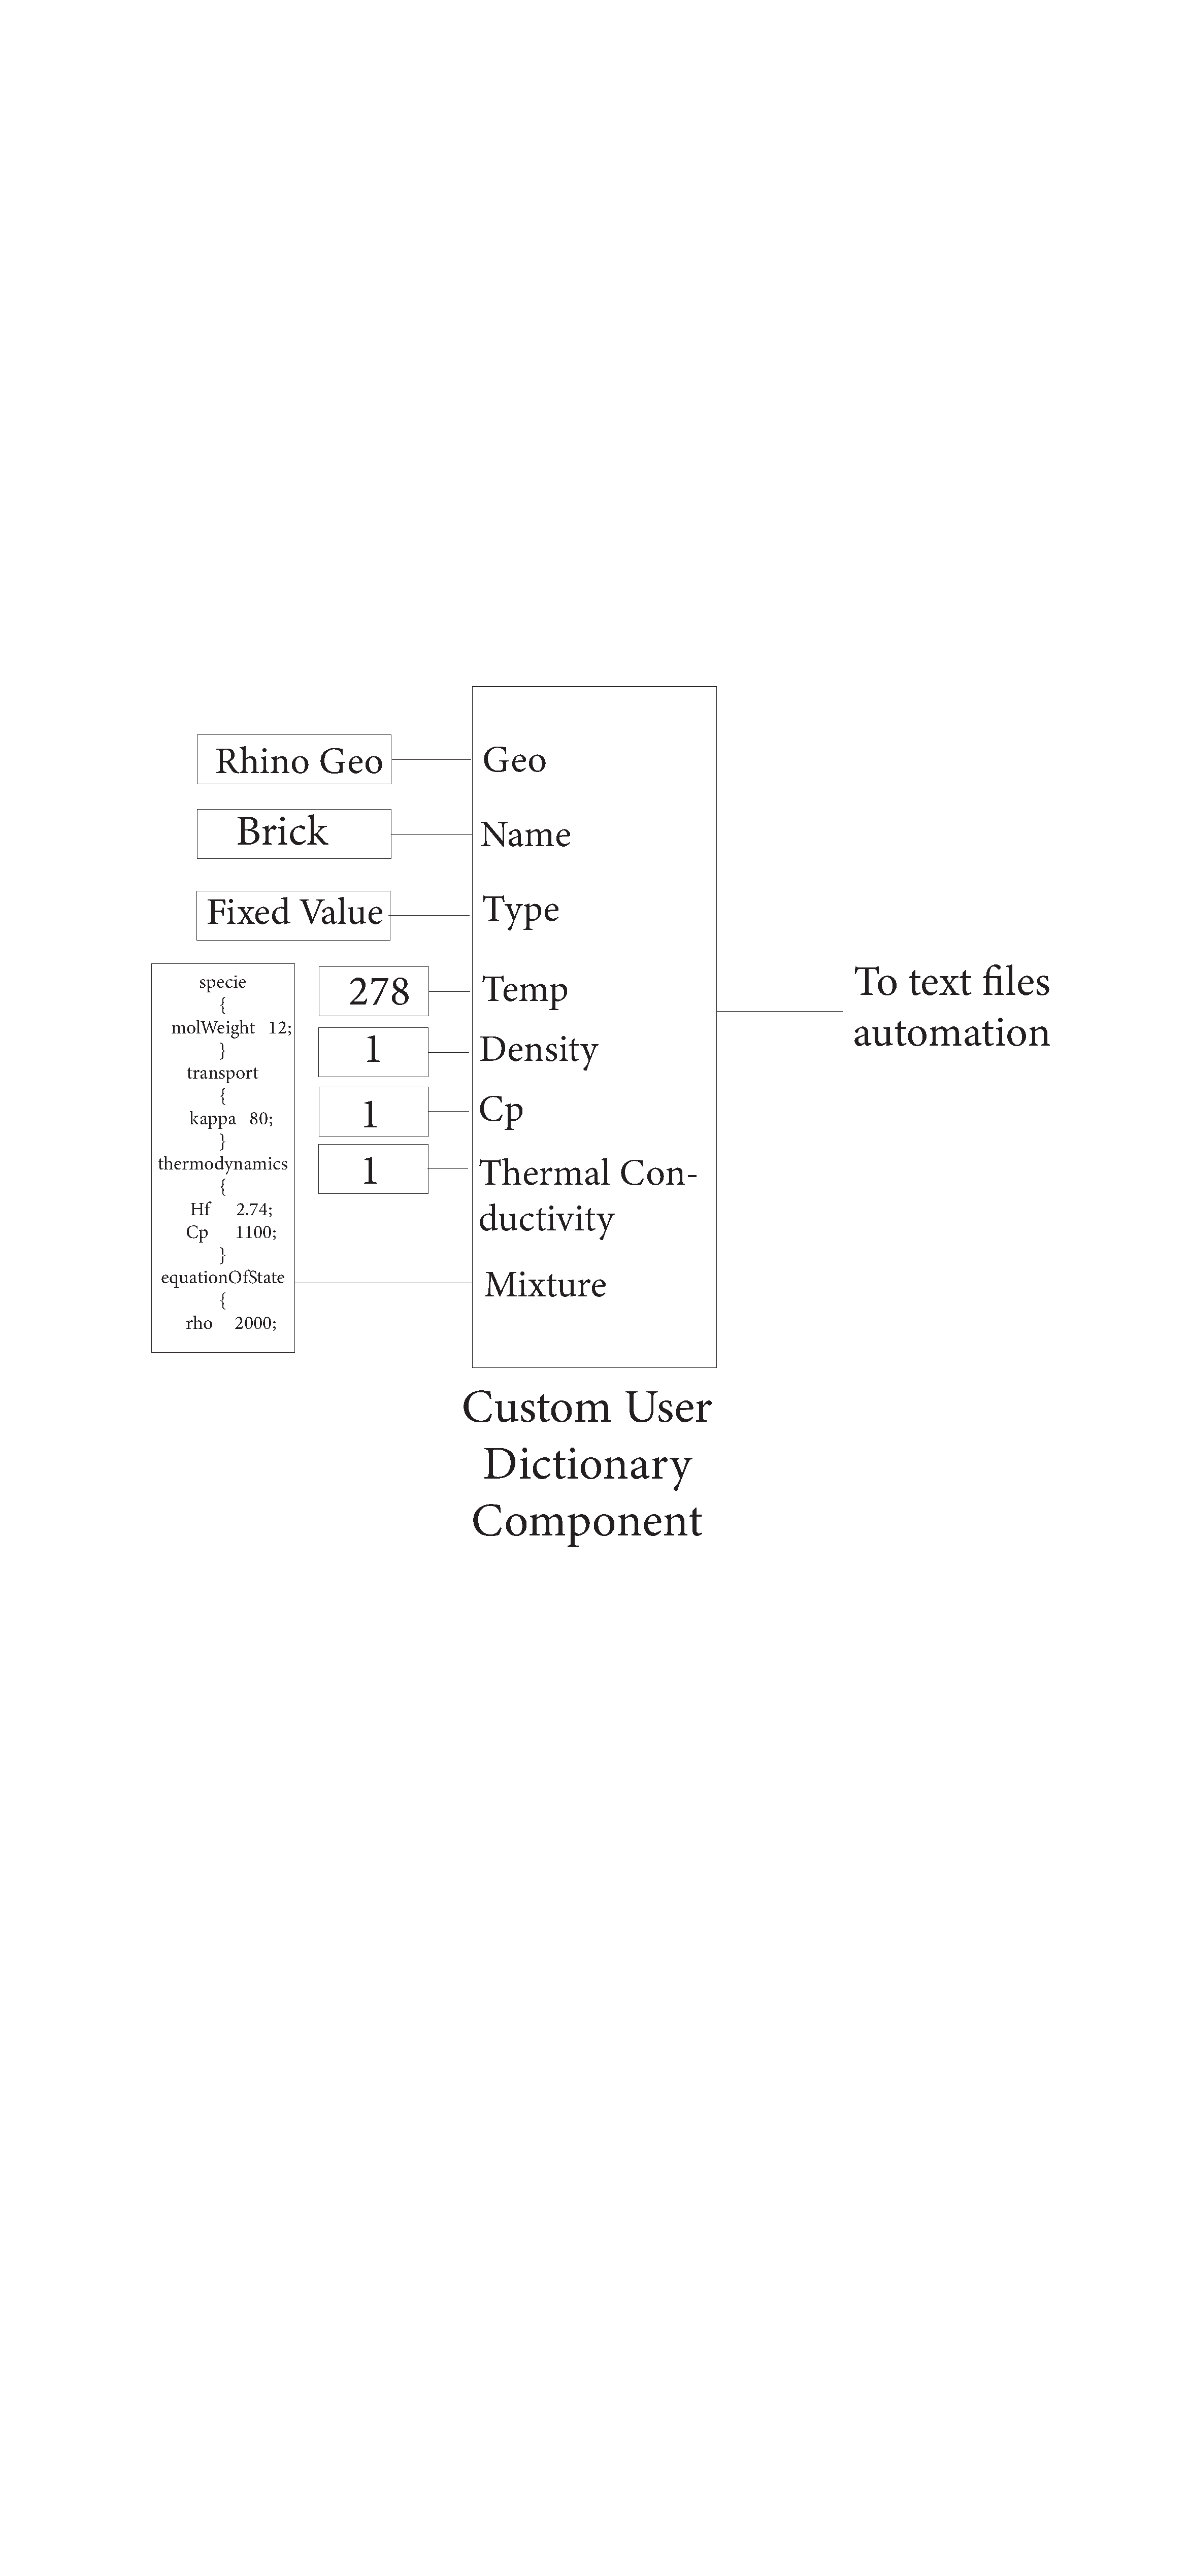
\includegraphics[trim=5cm 32cm 4.5cm 7cm, clip, width=0.55\linewidth]{Figures/THESISGH2.pdf}
\hspace{0.7cm}
\caption{\gls{GH} Material Properties Component.}
\label{matgh}
\end{figure}





\subsubsection{\gls{GH} Point in Mesh}
The workflow in \ref{locgh} automatically defines the point coordinates of each region of the mesh. Each region must have a point in Rhino, and the points each are connected to the corresponding material component. The \textit{locationInMesh} parameter identifies a specific point within the computational domain, allowing the \textit{snappyHexMeshtool} to identify and locate all cells connected to that point. This helps ensure that only certain regions/zones are kept during the mesh generation process, usually to separate different volumes or regions of interest.

In our case, one point is not enough to capture all 10 regions, so using \textit{locationsInMesh} is essential. This allowed us to specify a list of points that represent various locations within the mesh. Each point in this list creates a separate cell zone located in the \textit{constant/ConcreteTop/polyMesh/cellZones} file, allowing more complex meshing and region differentiation. This flexibility is useful for our case and for other complex geometries within a single mesh.

\begin{figure}[tb]
\centering
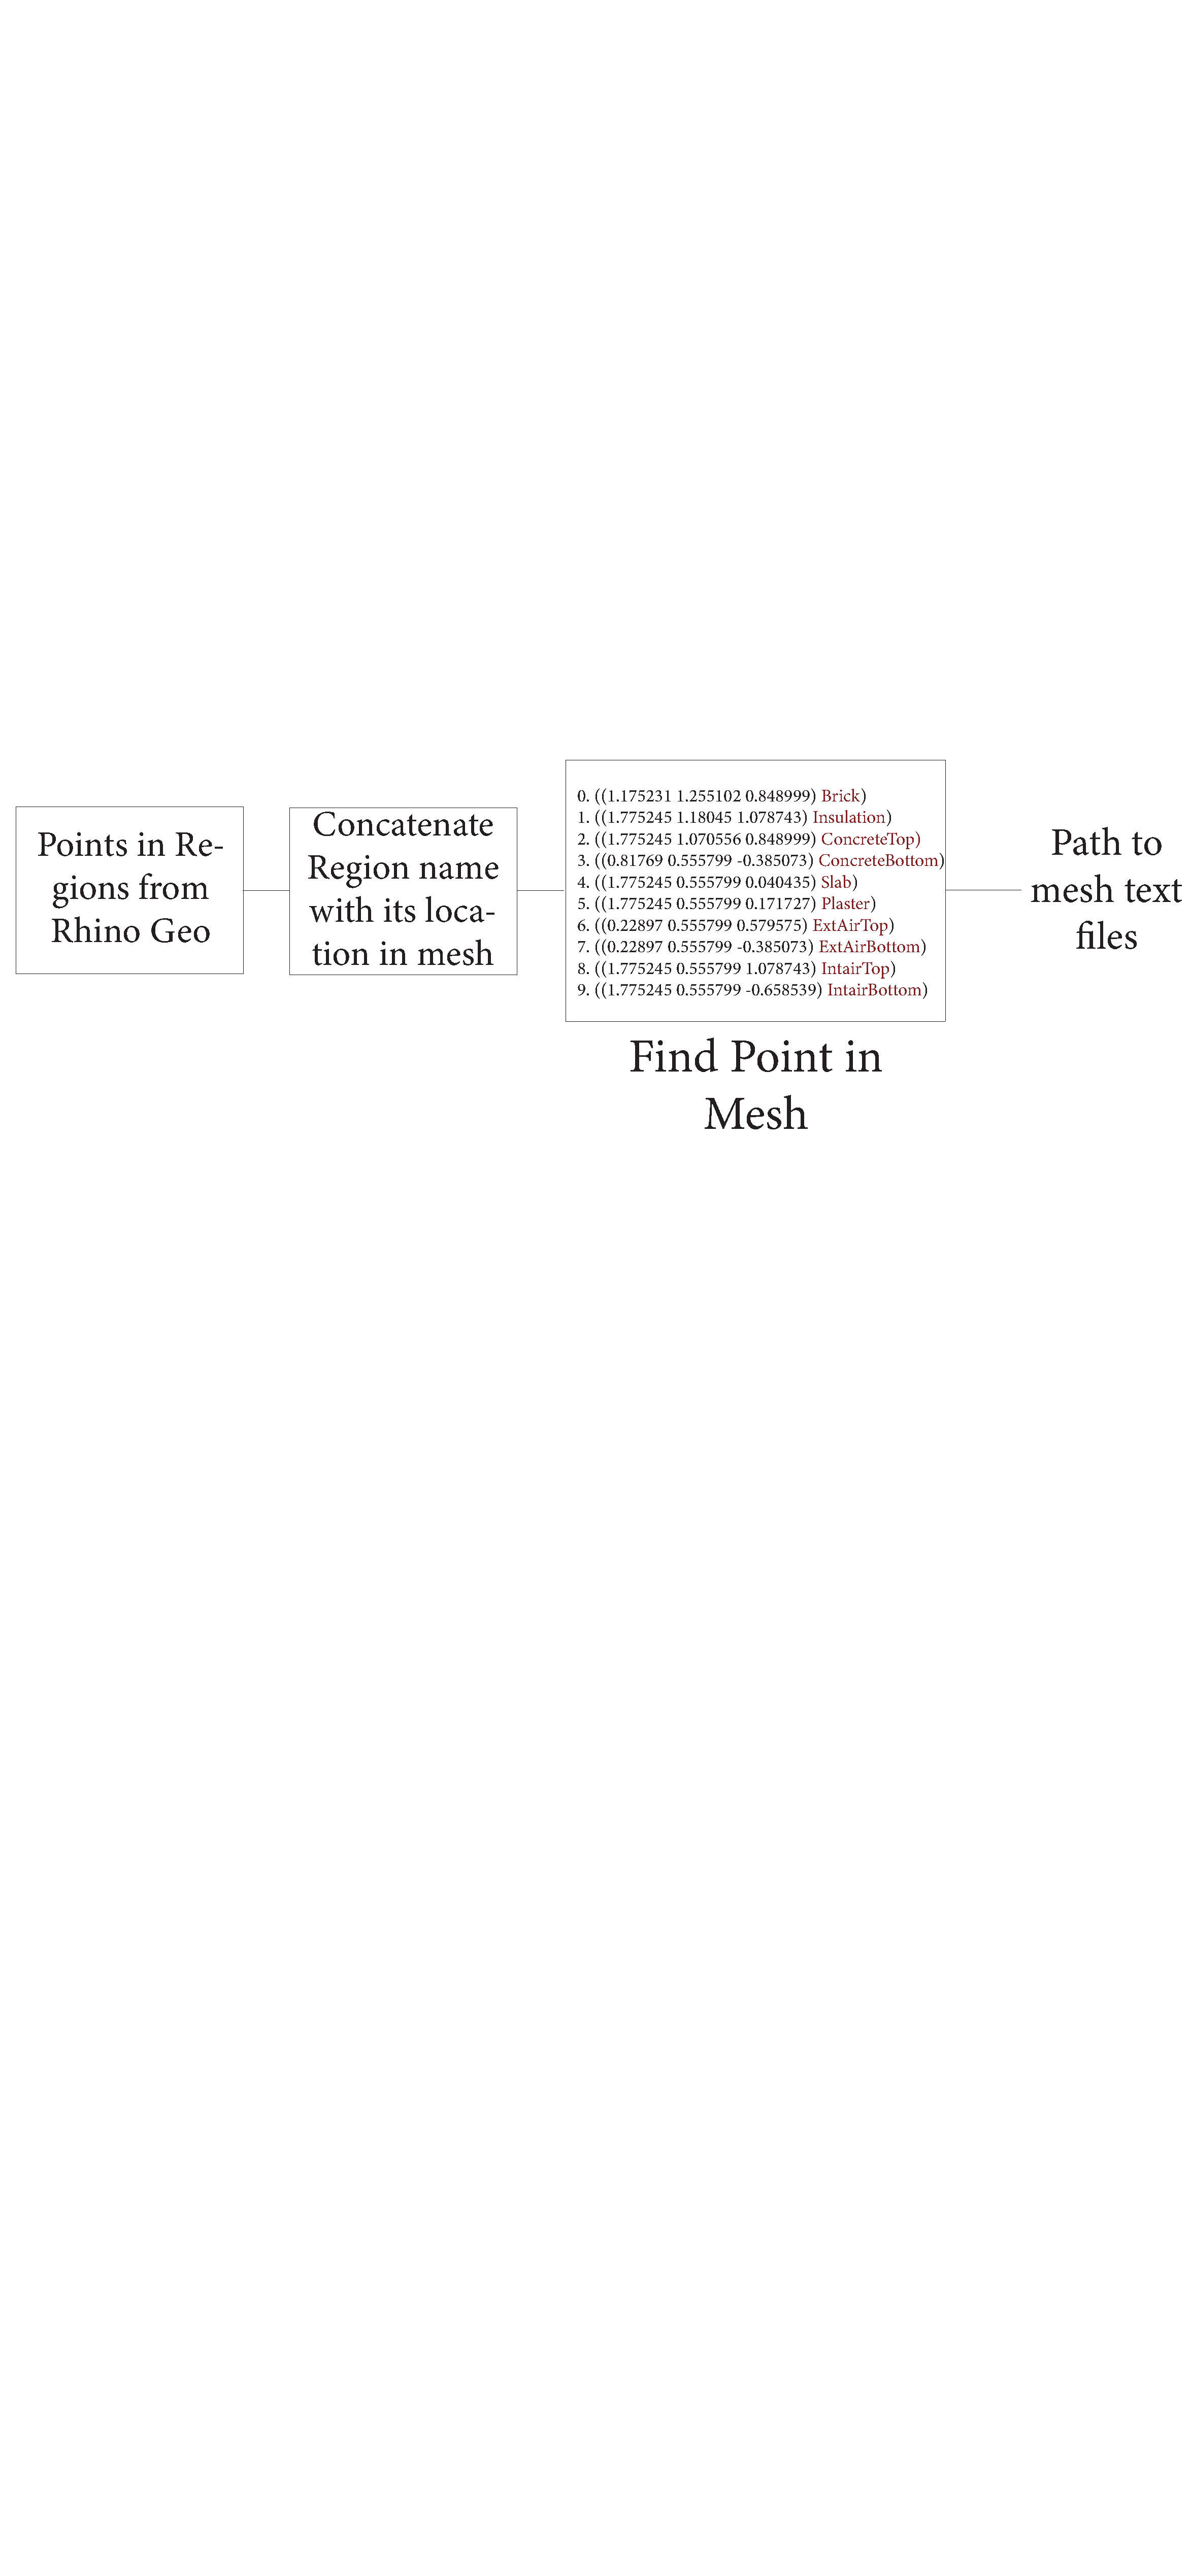
\includegraphics[trim=0cm 45cm 0cm 24cm, clip, width=0.8\linewidth]{Figures/locinmeshgh.pdf}
\hspace{0.7cm}
\caption{\gls{GH} Point in Mesh Workflow.}
\label{locgh}
\end{figure}








\subsubsection{Surface Combinations}
The surface combinations workflow shown in \ref{surfgh} writes the zone interfaces to be used in each zone text file in \textit{constant}, \textit{system}, and \textit{0}. 

\begin{figure}[tb]
\centering
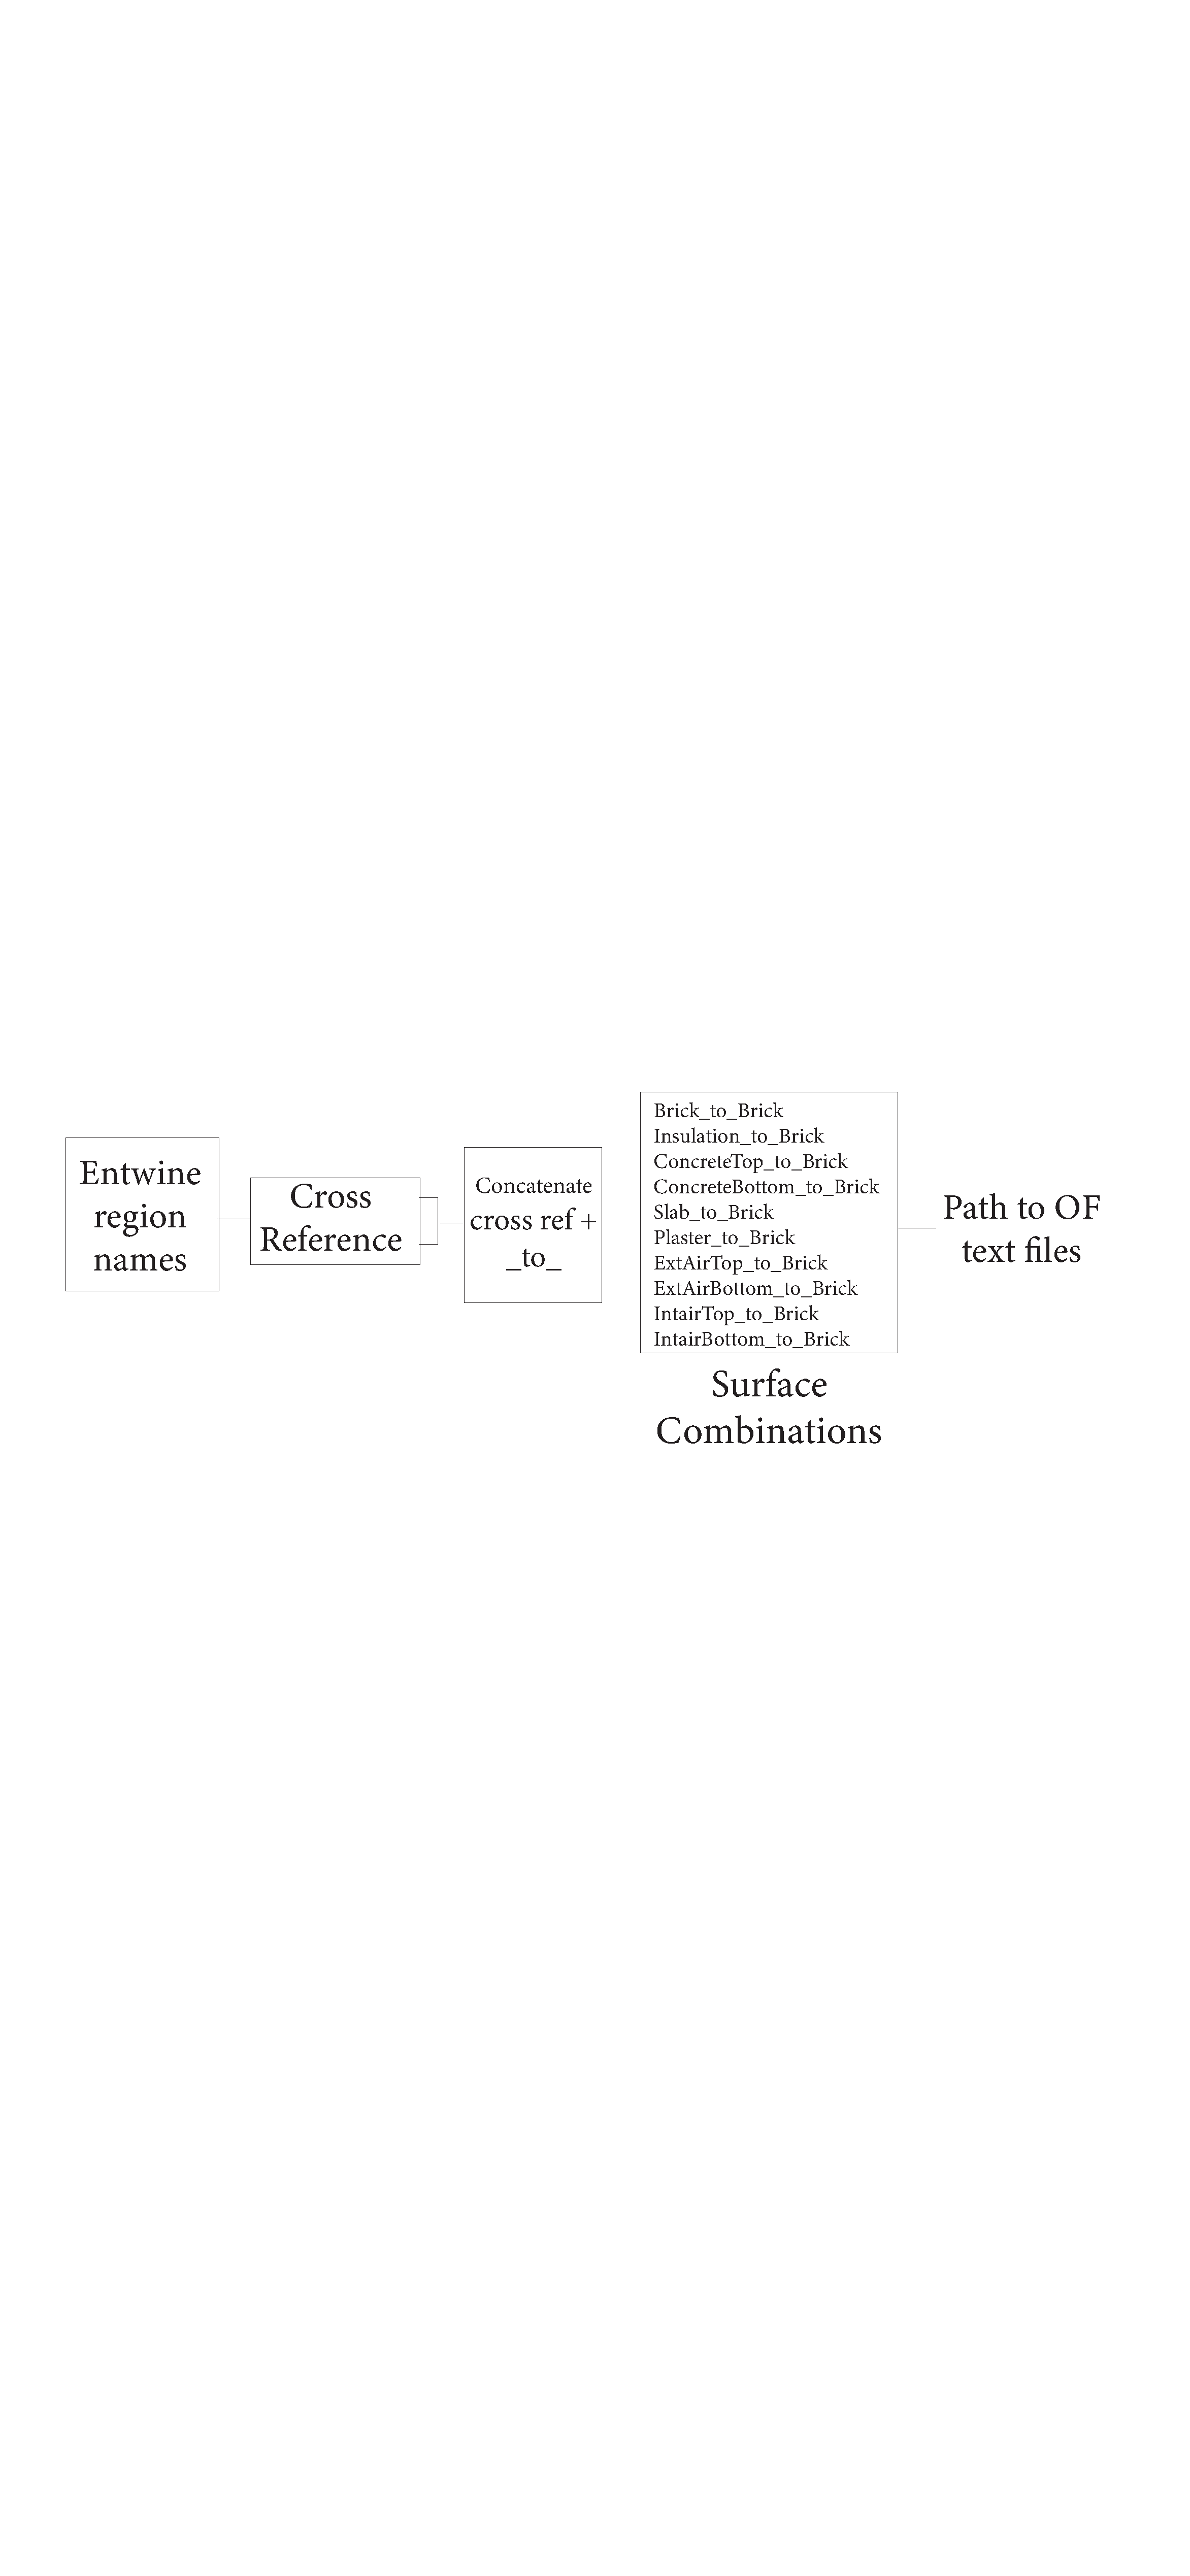
\includegraphics[trim=0cm 39cm 0cm 29cm, clip, width=0.8\linewidth]{Figures/surfcombgh.pdf}
\hspace{0.7cm}
\caption{\gls{GH} Surface Combinations Workflow.}
\label{surfgh}
\end{figure}



\subsubsection{Write p File Example}
The \gls{GH} script includes sections to write all of the $p$, $T$, $U$, and properties files needed to run the simulation for each zone. All other required text files, such as T and U, are written using the same workflow where the component includes a script that writes the text file in the required format \gls{OF}. Furthermore, all the necessary boundary conditions and material specifications are taken from the material dictionary component in \cref{matgh}.


















\section[OpenFOAM]{OpenFOAM (OF)}
As briefly stated at the beginning, this project utilizes the CFD capabilities of OpenFOAM (Open-source Field Operation and Manipulation, or OF).  \gls{OF} is a C++ toolkit built for developing custom numerical solvers and pre- and post-processing tools. \gls{OF} is mainly used to simulate computational fluid dynamics (CFD). The software is open-source, free to use, and distributed under the GNU General Public License Version 3.
By integrating the capabilities of \gls{OF} into Rhino, the complexity of setting up a 3D heat transfer case is simplified and minimized. When using OpenFOAM for simulations, it is important to note that the temperatures for boundary conditions must be specified in Kelvin.

This section provides a detailed description of the case's pre-processing, case study setup, selected solver, and physical models, as well as a description of constructing and running the case. 
Finally, it provides detailed post-processing steps.



\subsection{Pre-processing}
The pre-processing phase consists of dividing the geometry into different zones based on different materials and locations. In addition, thermophysical properties, such as specific heat capacity and thermal conductivity, are assigned to the materials, and fluid or solid properties are assigned to regions. The limit conditions and the construction materials are specified in \cref{fig:validation-case-materials} \textbf{(a)} and \textbf{(b)}. 


\begin{figure}[h!]
    \centering
    \begin{minipage}[t]{1\columnwidth}
        \centering
        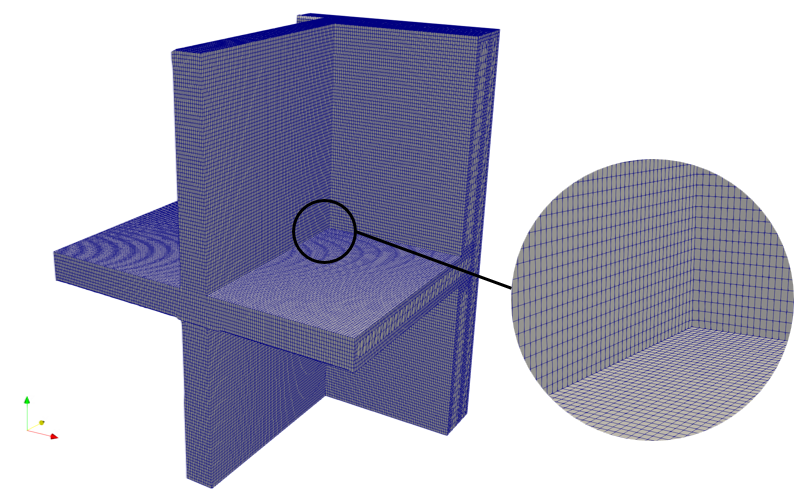
\includegraphics[width=\linewidth]{Figures/mesh3.png}        
        \subcaption*{\textbf{(a)}}
        \vspace{0.5cm}
    \end{minipage}
    
    \begin{minipage}[t]{0.5\columnwidth}
        \centering
        \begin{tabular}{clrrr}    
            \toprule
            & Type       & Multi-block dataset   \\ \midrule
            & \# of Cells & 360,364                      \\
            & \# of Points                        & 3,481,036                  \\
            & \# of TimeSteps                  & 400                        \\
            & Bounds X          & 0 to 1.9 (delta: 1.9) \\
            & Bounds Y          &                     0 to 1.25 (delta: 1.25) \\
            & Bounds Z          &                     -1 to 1.15 (delta: 2.15)    \\  \bottomrule
        \end{tabular}
        \caption*{\textbf{(b)} 3D Validation case mesh statistics.}
        \label{tab:mesh-stats}
    \end{minipage}
    
    \caption[3D Validation Mesh and Mesh Statistics]{\textbf{(a)} \gls{OF} mesh viewed in ParaView without air regions. \textbf{(b)}  Validation case mesh statistics retrieved from ISO 10211:2007 (E) \cite{ISO}.}
    \label{fig:validation-case}
\end{figure}






\begin{table}[tbh]
    \centering
    \label{tab:construction_material_properties}
    \caption[3D Material Properties]{Construction material properties and boundary conditions used for the simulation domain. Data were taken from the demo example in QuickField.}
      \centering
        %\footnotesize
        \begin{tabular}{clrrr}    
            \toprule   
            & Materials       & $k$ $\left[ \si[per-mode=fraction]{\watt\per\metre\kelvin} \right]$ & $c_p$   $\left[ \si[per-mode=fraction]{\joule\per\kilogram\kelvin}\right]$ & $\rho$  $\left[ \si[per-mode=fraction]{\kilogram\per\cubic\metre} \right]$   \\
            \midrule
            & Floor Slab        & 2.5                        & 1000                      & 2300               \\
            & Aerated Concrete  & 2.5                        & 1000                      & 2300               \\
            & Brick             & 0.7                        & 1060                       & 710               \\
            & Insulation        & 1                         & 1450                      & 35               \\
            & Plaster           & 1                         & 1000                      & 2300              \\
            \bottomrule
        \end{tabular}
  
\end{table}


    \begin{table}[tbh]
   
      \caption{3D Boundary Conditions}
      \centering
        %\footnotesize
        \begin{tabular}{llrr}    
            \toprule   
            & Boundary conditions          & $T [\si{\degreeCelsius}]$           & BC type                   \\ 
            \midrule
            & Inside temp.  (1st floor)         & 20                          & fixedValue                \\
            & Inside temp.  (2nd floor)          & 15                          & fixedValue                \\
            & Outside temp.  & 0                          & fixedValue                \\ 
            \bottomrule
        \end{tabular}

\end{table}






\subsubsection{Case Study setup}
The case study geometry was exported from QuickField and then modeled in Rhinoceros and subsequently exported as a mesh to be processed with  \gls{OF} where \ref{meshsteps} visualizes the steps to create the mesh. 
The validation case was constructed in \gls{OF} by creating the mesh and \textit{snappyHexMesh} files.  
\ref{fig:validation-case-materials}  (b) illustrates the \gls{OF} mesh visualized in ParaView.
    



%\clearpage
\subsection{Simulation Equations}

\subsubsection{Solver Setup}
The solver used in this case is \textit{chtMultiRegionFoam} in  \gls{OF} 2306 which is a solver capable of solving for steady or transient fluid flow with solid heat conduction and conjugate heat transfer between regions, buoyancy effects, turbulence, reactions, and radiation modeling\footnote{Not used in this study.} \cite{cht}.
There are three solvers capable of simulating steady-state heat transfer between fluids and solids which are \textit{chtMultiRegionFoam}, \textit{chtMultiRegionSimpleFoam}, and \textit{chtMultiRegionTwoPhaseEulerFoam}, but, the key distinction is that the selected solver for this case is capable of doing both steady and transient states to have a more versatile and adaptable software depending on the application. 


To precisely mimic real-world situations, the use of \textit{ chtMultiRegionFoam} solver is essential to have accurate 3D heat transfer results due to the availability of using fluid and solid. \Cref{interface} visualizes the capabilities of the solver with the various domains and interfaces of different temperatures, solids, and fluids. 
A description of the boundary conditions can be found in \cref{tab:construction_material_properties}. 
However, the outdoor temperature is set to be 0°C and the climate boundary condition setup could be easier by using Grasshopper to leverage the initial temperatures based on the location. 
Another crucial aspect is identifying the thermal properties that will allow the solver to identify the thermal conductivity, density, and properties of the material and calculate the heat transfer accordingly.

\subsubsection{CHT Solver Equations}    

This section presents the implementation of heat transfer equations and metrics in \gls{OF} and the solver from \gls{OF} Foundations \cite{OpenFOAMFoundation}.
\subsubsection{1. Fluid Equations}

Mass Conservation is:
\begin{equation}
\frac{\partial \rho}{\partial t} + \frac{\partial (\rho u_j)}{\partial x_j} = 0
\end{equation}


     

\subsubsection{2. Solid Equations}
Solid Energy Conservation is:

\begin{equation}
\frac{\partial (\rho h)}{\partial t} = \frac{\partial}{\partial x_j}\left( \alpha \frac{\partial h}{\partial x_j} \right)
\end{equation}

Where \( h \) is the specific enthalpy, \( \rho \) is the density, and \( \alpha = \frac{\kappa}{c_p} \) is the thermal diffusivity, and the specific heat capacity \( C_p \).


\subsubsection{3. Solid and Fluid Interface}
\begin{equation}
T_f = T_s  \\
Q_f = -Q_s  \\
\kappa_f \frac{d T_f}{d n} = -\kappa_s \frac{d T_s}{d n} 
\end{equation}

Where \( \kappa_f \) thermal conductivity of the fluid and \( \kappa_s \)  the thermal conductivity of the solid.







\subsection{Physical Models}
The physical models found in the constant file are required for the simulation to run according to the \gls{OF} documentation \cite{OFD}. However, it is also an important part in the integration of architecture and building geometry. First, the \textit{turbulence model} is connected to the fluid in the space, and the fluid properties. \textit{Turbulence} is useful when understanding the thermal comfort in space, but also to combine the conduction of the interaction of the material in the interface with the convection to have an accurate heat transfer result. Moving to the second physical model, which is the \textit{ thermophysical model}, where its connection to architectural modeling is to specify each of the properties of the material used to accurately understand the rate of heat transfer. Finally, moving to the last model, which is the \textit{finite volume options model} which includes required models such as turbulence and optional models to provide additional detailed boundary conditions and specify the heat sources. 
This option can be used in architectural applications to optimize for the best location of the heat source or other specific limits. The following is a detailed description of each of the physical models in OpenFOAM.


\subsubsection{Turbulence Properties}
The turbulence used for steady-state heat transfer is \gls{RAS}, where the full form is an anisotropic contribution of Reynolds stress, shown below, to influence the motion of a fluid, providing a comprehensive understanding of fluid flow dynamics. Where the heat conservation equation according to \cite{hce}:

\begin{equation}
u_i \frac{\partial T}{\partial x_i} + \frac{\partial}{\partial x_i}(K_T \frac{\partial T}{\partial x_i}) = 0 \label{eq:heat}
\end{equation}

Where \(u_i\) is the velocity component in the \(i\) direction, \(T\) is the temperature, \(x_i\) is the spatial coordinate in the \(i\) direction, and \(K_T\) is the thermal conductivity coefficient.

The Navier-Stokes equation describes the conservation of momentum for a fluid:

\begin{equation}
\frac{\partial (\rho u_i)}{\partial t} + \frac{\partial}{\partial x_j} \left( \rho u_i u_j \right) = -\frac{\partial p}{\partial x_i} + \frac{\partial}{\partial x_j} \left( \tau_{ij} + \tau_{t_{ij}} \right) + \rho g_i
\end{equation}

Where \(\rho\) is the fluid density, \(u_i\) is the velocity component in the \(i\) direction, \(t\) represents time, \(p\) is the pressure, \(\tau_{ij}\) is the viscous stress tensor, \(\tau_{t_{ij}}\) is the turbulent stress tensor, and \(g_i\) represents the body force in the \(i\) direction (such as gravity).


Where, $\rho$ is the density of the fluid, $u_i$ is the velocity component in the $i$-direction, $t$ is time, $x_i$ is the spatial coordinate in the $i$-direction, $p$ represents pressure, $\tau_{ij}$ is the viscous stress tensor, $\tau_{t_{ij}}$ is the turbulent stress tensor, and $g_i$ is the gravitational acceleration in the $i$-direction
 \cite{cht}.


\subsubsection{Thermophysical Models}
The thermophysical properties located in each zone and the constant file require input of density $\rho$, thermal conductivity, and specific heat capacity for every material.
\subsubsection{Finite Volume Options}
The fvOptions text file allows the user to further manipulate the systems of equations, such as sources and sinks \cite{ofvoptions}.  


\subsection{Constructing The Case}    
An \gls{OF} steady state heat transfer case requires three main folders to run, namely iteration \textit{0}, \textit{constant}, and \textit{system} folders. Each folder is responsible for properties or boundary conditions and includes these conditions in each zone in the geometry. The 10 zones in the case which are \textit{Brick}, \textit{Slab}, \textit{Plaster}, \textit{ConreteTop}, \textit{ConreteBottom}, \textit{IntAirTop}, \textit{ExtAir}, \textit{IntAirBottom}, \textit{InsulationTop}, and \textit{InsulationBottom}. Below in \cref{constc} is an explanation of the case contents. The text files in this case are written automatically due to the script setup in \gls{GH}. While creating the constant file, the specific heat capacity of each material was needed, so we followed the steps in \ref{appendcp} in the appendix to estimate it.






\begin{figure}[tb]
\centering
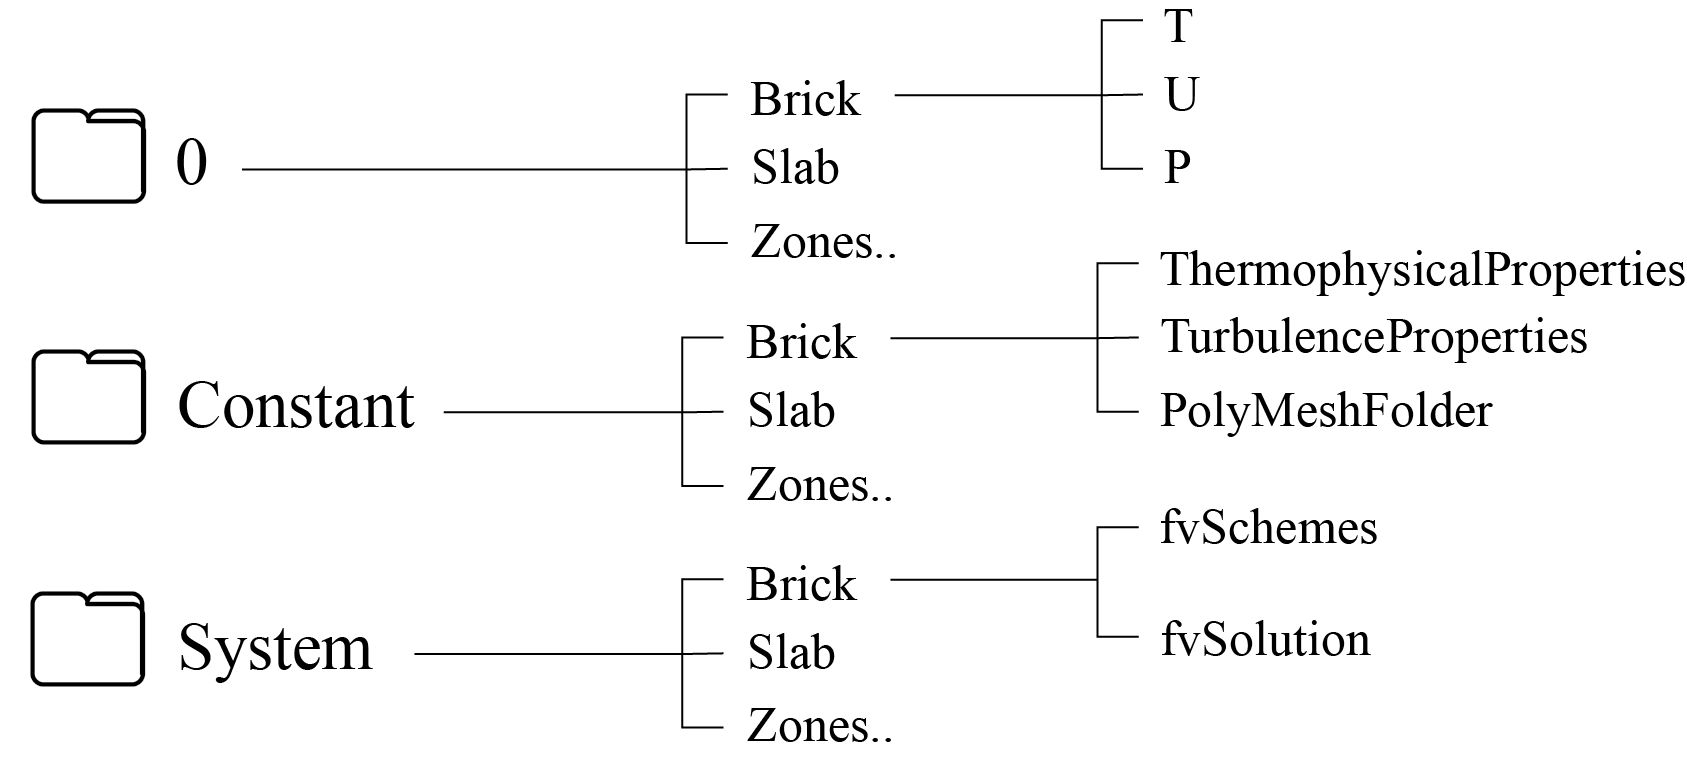
\includegraphics[width=0.77\columnwidth]{Figures/constc.png}
\hspace{0.7cm}
\caption[OF Case Contents]{OF case folders to run. Where (zones..) represent a folder for each zone in the case.}
\label{constc}
\end{figure}





\subsection{Running The Case}    
 
After discussing the selected solver capabilities to run the numerical simulation. The goal is to solve heat transfer in solid and liquid regions between air regions and the selected geometry. Using the software QuickField to solve for 3D heat transfer showed some limitations where it does not consider the air regions. However, our approach using  \gls{OF} includes the integration between air and solids to produce more accurate results. 

\begin{figure}[tbh] 
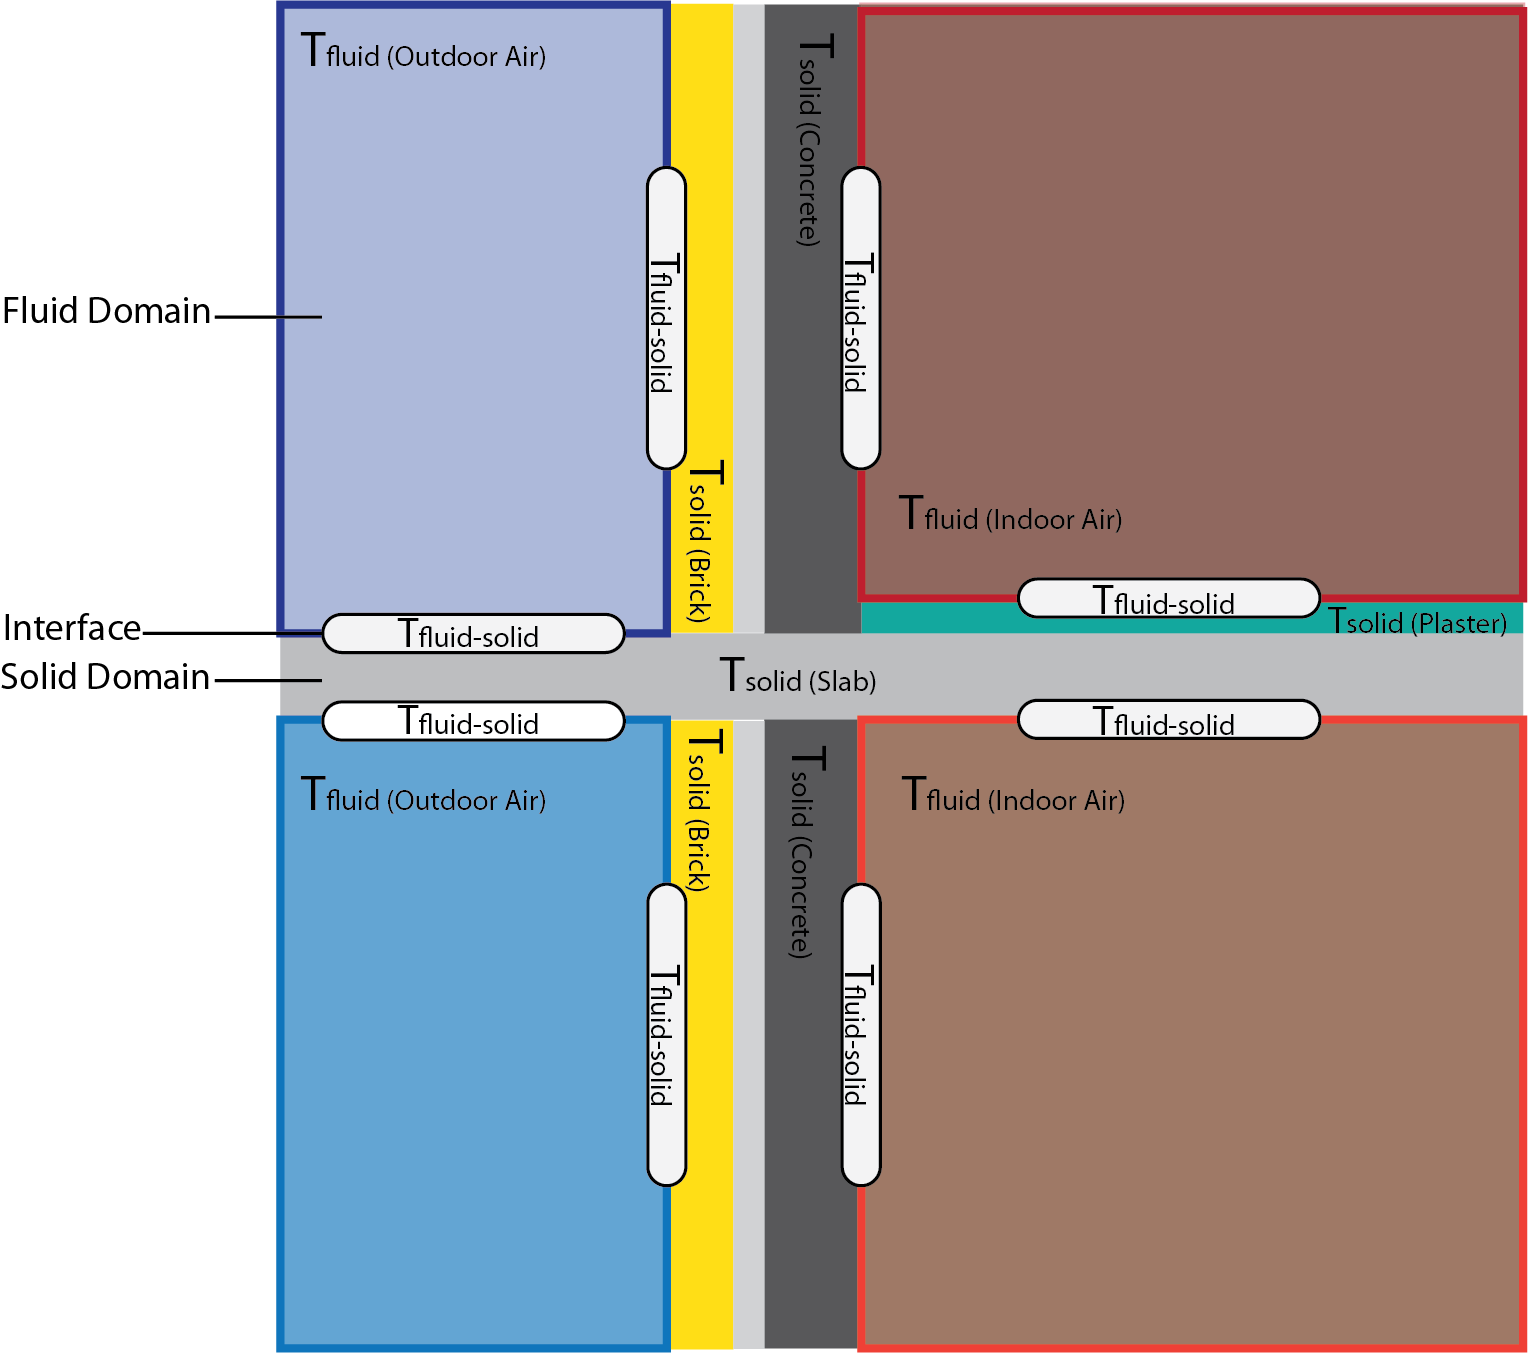
\includegraphics[width=0.77\columnwidth]{Figures/conductive.png}
\hspace{0.7cm}
\caption[3D Interfaces]{Vertical section of the validation case shows convection and conduction.}
\label{interface}
\end{figure}

\begin{figure}[tbh]
\centering

\begin{tikzpicture}[node distance=1.55cm, thick, every node/.style={scale=1}]
% Define nodes
\footnotesize
\node (blockMesh) [block] {blockMesh};
\node (surfaceFeatureExtract) [block, below of=blockMesh] {surfaceFeatureExtract};
\node (snappyHexMesh) [block, below of=surfaceFeatureExtract] {snappyHexMesh};
\node (splitMeshRegions) [block, below of=snappyHexMesh] {splitMeshRegions};
\node (chtMultiRegionFoam) [block, below of=splitMeshRegions] {chtMultiRegionFoam};
% Connect nodes with arrows
\draw [arrow] (blockMesh) -- (surfaceFeatureExtract);
\draw [arrow] (surfaceFeatureExtract) -- (snappyHexMesh);
\draw [arrow] (snappyHexMesh) -- (splitMeshRegions);
\draw [arrow] (splitMeshRegions) -- (chtMultiRegionFoam);
\end{tikzpicture}


\caption[OF Executables]{Order of executables for multiregion case setup with  \gls{OF} v2306.}
\label{fig:order-of-executables}
\end{figure}






\ref{fig:order-of-executables} illustrates the executables that need to be executed in order for a multiregion case.
The \textit{blockMesh} utility generates parametric meshes incorporating grading and curved edges. 
The meshes are created based on the specifications outlined in a dictionary file named \textit{blockMeshDict}  within the case directory.
\textit{surfaceFeatureExtract} extracts the surface features and then records them in a file.      
\textit{snappyHexMesh} is a utility in \gls{OF} that generates 3D meshes with hexahedra from STL surfaces, iteratively refining while maintaining surface conformity, shown in \ref{meshsteps}.
\textit{splitMeshRegions} divides the mesh into separate regions. Each region consists of cells reachable without crossing boundary faces, including cell zones.
\textit{chtMultiRegionFoam} is a solver for both steady and transient fluid flow, with solid heat conduction and conjugate heat transfer. The equations for each system variable are solved, and the solutions from the preceding equations are inserted into the subsequent ones. For instance, fluid-solid coupling solves fluid equations first, using the previous iteration's solid temperature to set fluid temperature boundary conditions. Then we solved the fluid equations using the same method. The simulation using this process continued until convergence at time step 400.
    
\begin{figure}[htb]
     \centering
    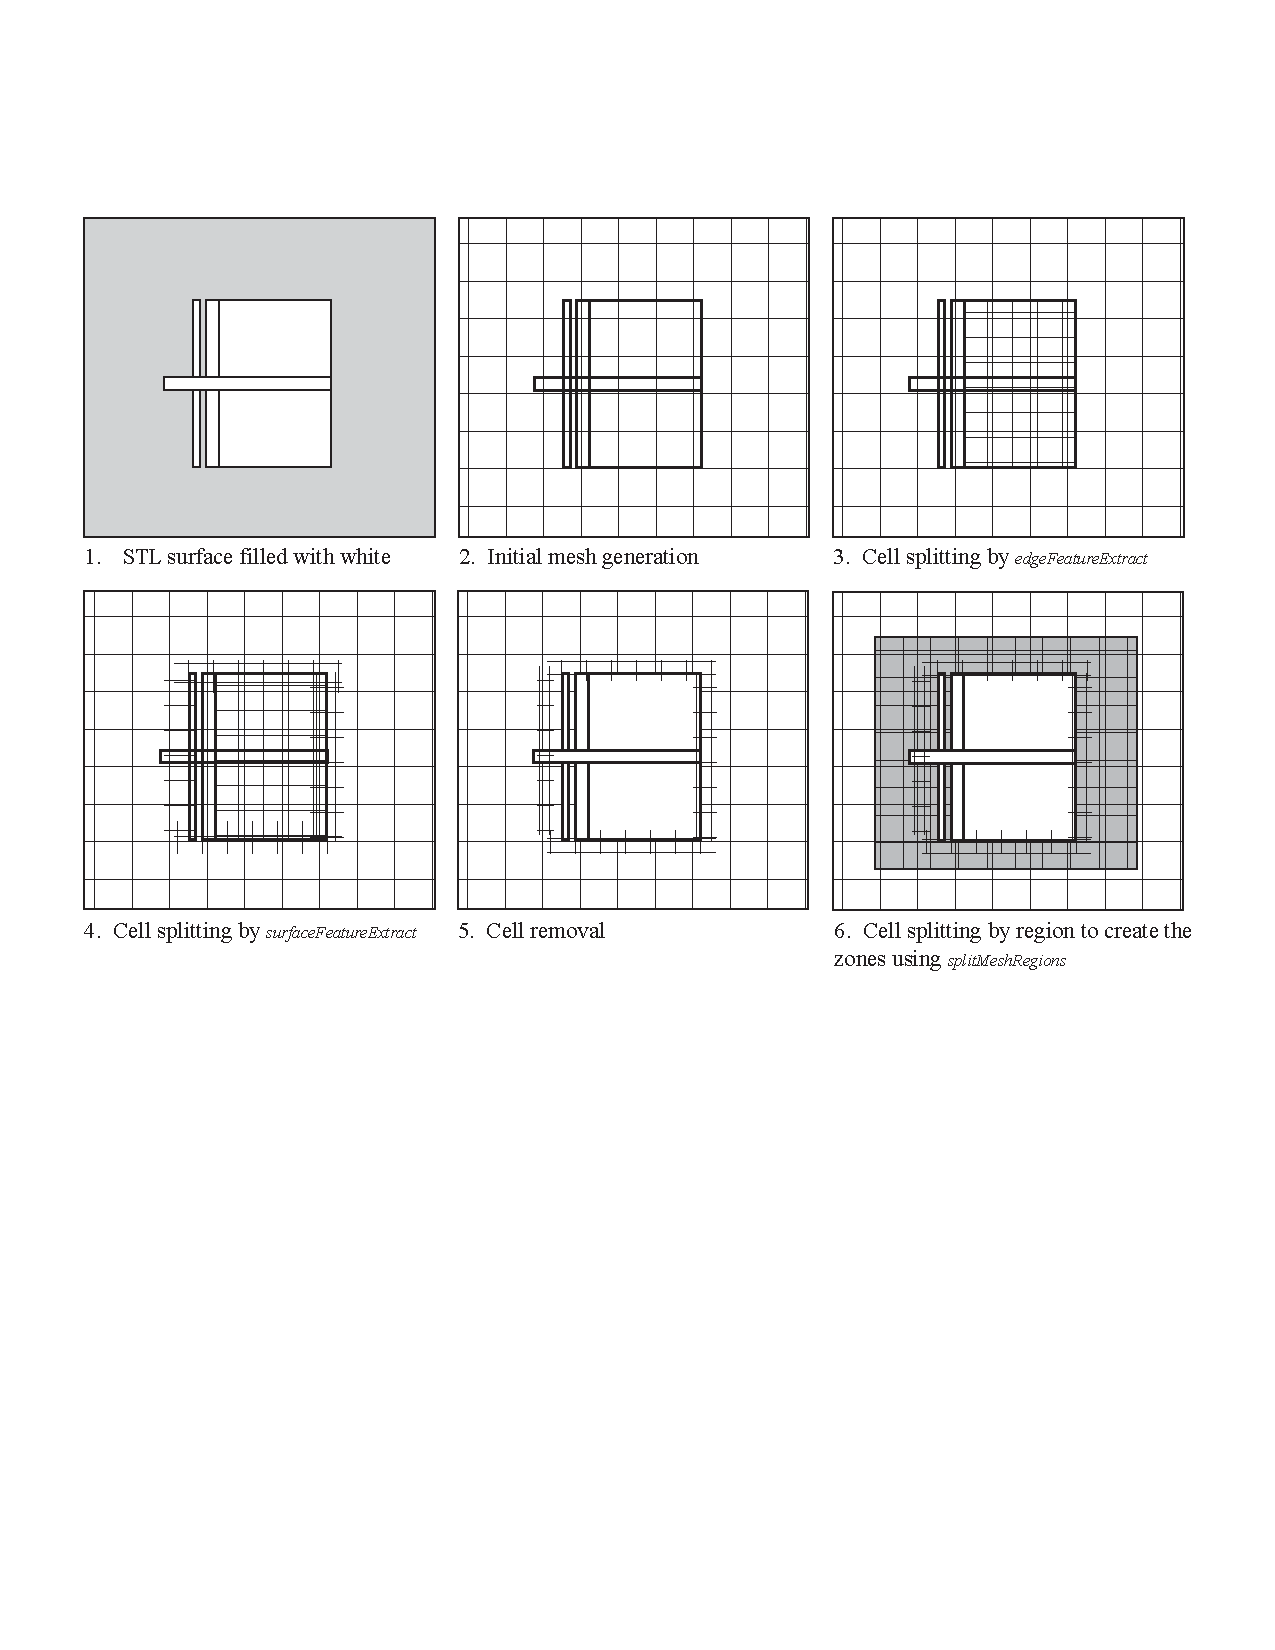
\includegraphics[trim=1cm 11cm 1cm 3cm, clip, width=1\linewidth]{Figures/snappyhex.pdf}
     \caption[Mesh Creation Steps]{Visualization of the steps and executables to create the mesh step-by-step.}
   \label{meshsteps}
 \end{figure}


%\clearpage
\subsection{Post-processing}
After running the simulation until convergence, multiple text files of $T$, $P$, and $U$ are solved for each region. There are two methods to post-process and visualize the resulting data. The first method is using Paraview to visualize the outcome and process the results. The second method is \gls{OF}'s post-process command, first, select the probing locations using \gls{GH} automation components to automatically write the post-processing file and measure the data, then plot the data to compare the validation case temperatures with our results. 



\afterpage{\clearpage}
\section{Results}

This section discusses the results of key experimental results of our ongoing research. 
\Cref{paraview} \textbf{(a)} visualizes the simulation temperature output, including the air (fluid) regions. Whereas
\Cref{paraview} \textbf{(b)} shows the geometry excluding air, which represents the temperature distributions. The resulting temperatures are shown in the plot in \cref{fig:validation-plots}. The plot includes the QuickField outputs and our \gls{OF} simulation along the z-axis from $z= 1.2$ to $z=2.2$ (the red line shown in \cref{paraview} \textbf{(a)}) and represents non-linear progression as a result of the different specific heat capacities and thermal conductivity of the materials. The peak in z=1.8 refers to the temperature of the slab, which can be modified by readjusting the slab model and re-simulating it. 



\begin{figure}[htb]
    \centering
    \textbf{(a)}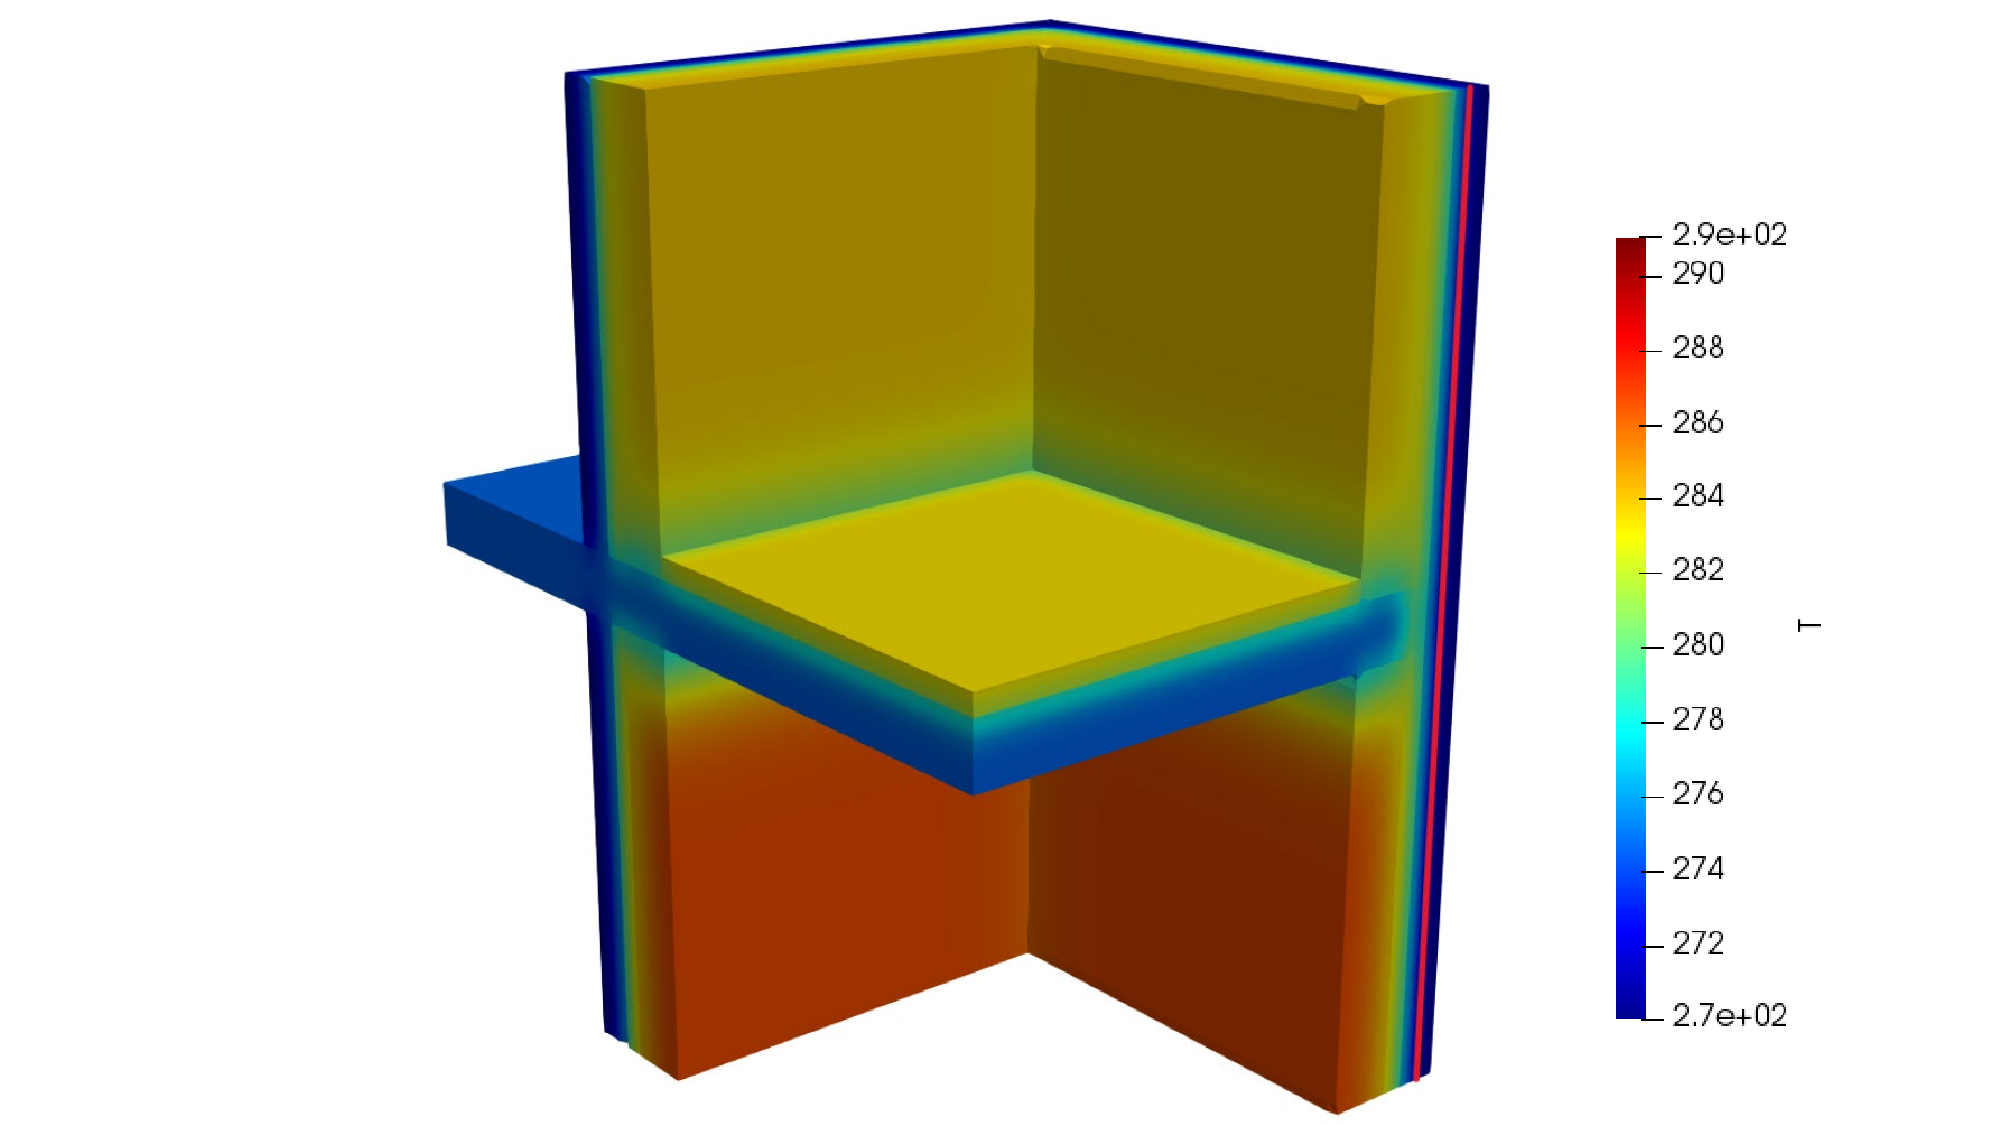
\includegraphics[trim=5cm 0cm 4.5cm 0cm, clip, width=0.70\linewidth]{Figures/newvalleg.pdf}
    \textbf{(b)}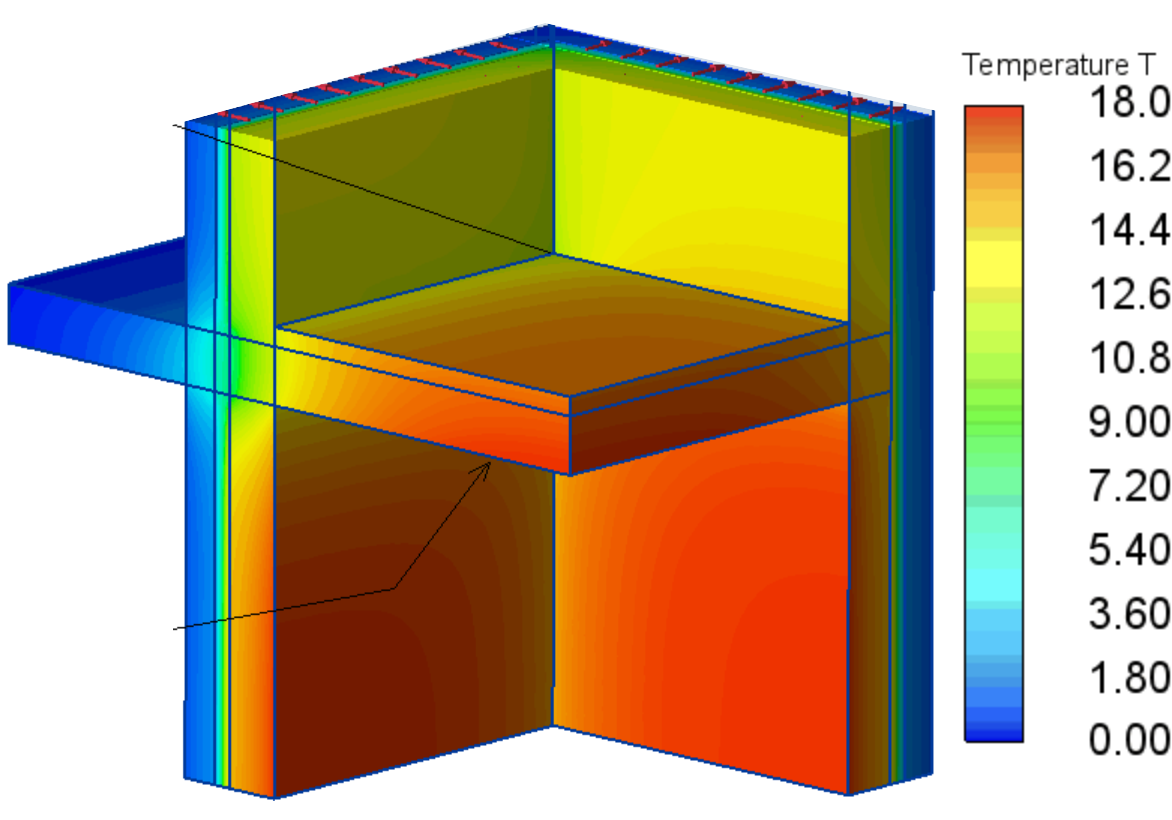
\includegraphics[width=0.65\columnwidth]{Figures/ValidationCaseClean.png}
\hspace{0.7cm}
    \caption[3D Validation Visualization]{\textbf{(a)} \gls{OF} case 3D results. \textbf{(b)} Quickfield validation results.}
    \label{paraview}
\end{figure}



\begin{figure}[htb] 
\centering
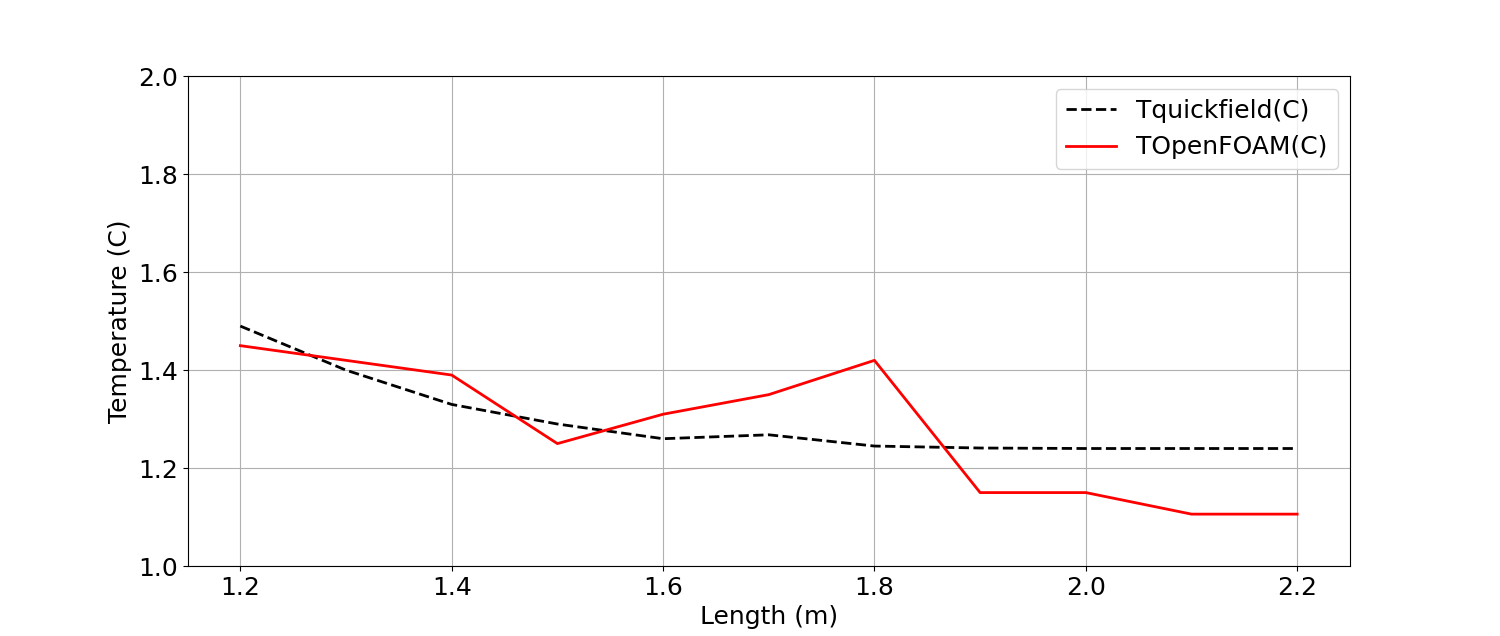
\includegraphics[width=1\columnwidth]{Figures/valpl2.png}
\hspace{0.7cm}
\caption{3D Validation Plots.}
\label{fig:validation-plots}
\end{figure}





\afterpage{\clearpage}
\section{Discussion}


The workflow presented in this thesis can be considered an extension of the work by \citeauthor{kastner2020solving} \cite{kastner2020solving}. 
The findings highlight several issues in the field, such as cost-prohibitive software, and disconnection between architectural modeling with heat transfer modeling software. 
The results illustrate the capabilities of using Rhinoceros and Grasshopper to simplify the pre-processing and post-processing steps to run the 3D heat transfer simulation in \gls{OF}. 
The simulation focuses on convective and conductive heat transfer for a 3D heat transfer problem. The 3D validation case study consists of two-floor corner sections separated by a concrete slab with a balcony. This case study was selected because it has the potential to present many challenges and problems in heat transfer, such as thermal bridges.


\subsection{Challenges}
\subsubsection{SIGFPE Error}
In some cases when changing or rescaling the geometry in Rhino, running the solver results in a signal floating-point error (SIGFPE), which might involve issues such as division by zero, floating-point underflow or overflow, integer overflow, etc. \cite{sigfpe}. However, in our case, the error occurs from divisions by zero and can be resolved in three ways depending on the circumstance. First, if the geometry in Rhino is re-scaled, the error can be resolved by recomputing the Grasshopper script. The second solution is to verify the boundary conditions in the $P$, and $P_{rgh}$ files, where they need to be absolute pressure and not relative when changing the \gls{OF} text files. The final solution is to recheck the boundary conditions and ensure that the zero gradient is properly assigned to the correct regions.


\subsubsection{Post-Processing}
Another challenge was to post-process the validation case via QuickField 6.6 (student version), which has several limitations compared to the \gls{OF} simulation discussed in this thesis. 
These include the inability to choose specific points to analyze temperature, limited visualization options, and no ability to adjust the density of points in the temperature plots. This made it difficult to compare specific temperature patterns.
QuickField 6.6 (student) does not allow selecting custom probing locations, limiting us to predefined ones.


\subsubsection{Slab Inaccuracy}
In the 3D validation case, the slab results demonstrate inaccuracies compared to the experimental case study. Despite the validation of the presented workflow of both the experimental design and the 3D case, the slab's behavior does not align as expected. An attempted solution involved changing the boundary condition at the $max_X$ boundary from $zeroGradient$ to $fixedValue$.
Although this adjustment slightly reduced the impact of the thermal bridge, it also introduced a larger issue by incorrectly representing heat transfer in the wall layer, as shown in Figure \ref{maxx}.

%gls/x, y, z

\begin{figure}[tb]
\centering
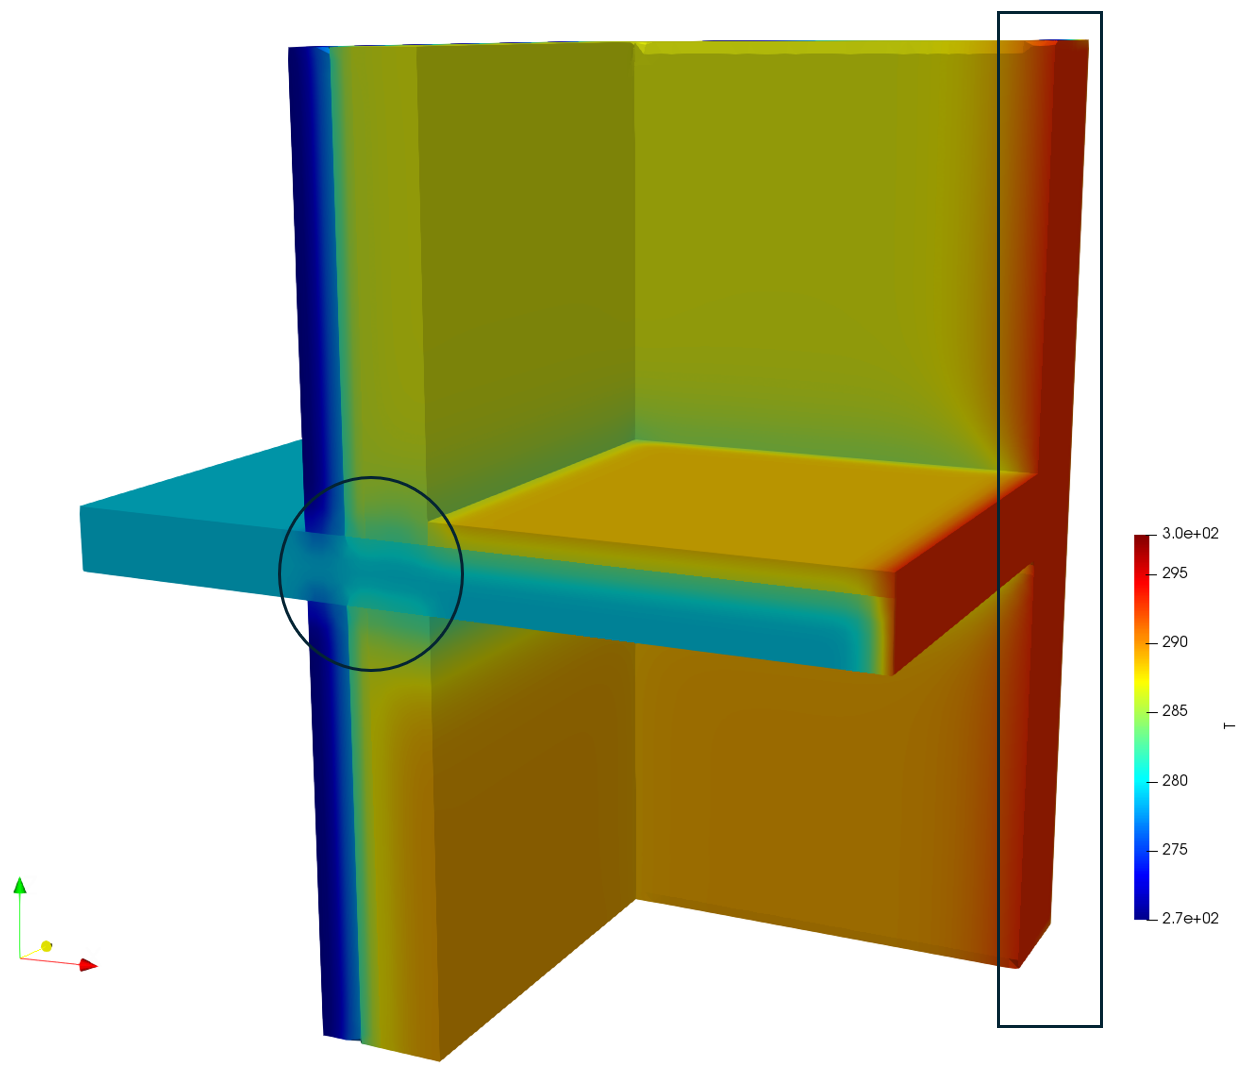
\includegraphics[width=0.75\columnwidth]{Figures/maxx.png}
\hspace{0.7cm}
\caption[Slab Validation]{Results of changing boundary conditions, highlighting a wall layer error and reduced thermal bridge.}
\label{maxx}
\end{figure}

Since these results do not fully consider the effect of thermal break between the exterior and interior sections of the slab, the following solutions may address the problem. The first suggested solution is to adjust the slab to have non-uniform initial conditions. This can be achieved by creating a $setFieldsDict$ file in the system folder. By using $setFieldsDict$, you can specify different initial temperatures for the exterior and interior sections of the slab, leading to a more accurate representation of the heat transfer. Another possible solution is to remodel the geometry and divide the slab into two distinct regions. This approach allows for better control over the thermal distribution and potentially improves accuracy in the simulation results.

Both of these solutions aim to correct the inconsistencies caused by incorrect boundary conditions and thermal bridging effects, leading to more accurate results in the 3D validation case.

\subsection{Experimental Design}
In the experimental design section of this thesis, U-value and heat flux sensors were used to log the temperatures and heat flux for a brick wall for 74 hours. The results were documented in 10-second increments throughout the three days. To validate the results of the experiment with the simulation \gls{OF}, three time steps were chosen from the experimental results to be simulated in three separate steady state heat transfer cases shown in \ref{table2d}, \ref{error2d}, and \ref{fig:expr}. However, the experiment can be easily validated by setting up one transient heat transfer case using the same \textit{chtMultiRegionFoam} solver. To leverage the solver's transient state capabilities, a time-dependent boundary condition must be provided. 


\subsection{Expanding Capabilities} %\todo{call this differently, this sounds weird}
Additional capabilities to the simulation is enabling the users to visualize the thermal comfort in the space (temperature of fluid in the space). Moreover, the use of the adaptable \textit{chtMultiRegionFoam} solver is designed to simulate complex heat transfer scenarios for various applications. It is suitable for analyzing and helping model the performance of heating and cooling systems in the HVAC  industry. In addition, the workflow can be used to assess solar heat gain, analyze heat exchangers, predict condensation, and assess insulation performance. Moreover, the integration into Rhino significantly reduces the time required to simulate 3D heat transfer by condensing the steps to achieve the simulation.



